\chapter{Loop tree \Author{S. Pop}}
\inputprogress
\graphicspath{{fig/}{loop_tree/fig/}{part3/loop_tree/fig/}}


\providecommand{\SSA}{SSA}
\providecommand{\CFG}{CFG}
\providecommand{\loopphi}{loop-$\phi$}
\providecommand{\closephi}{close-$\phi$}
\providecommand{\CHREC}[1]{\{#1\}}

This chapter presents an extension of the \SSA{} under which the
extraction of the reducible loop tree can be done only on the \SSA{}
graph itself.  This extension of the \SSA{} representation captures
more than the scalar computations: the phi nodes and the scalar
assignments encode the strongly connected components of the CFG that
are the reducible loops.  This chapter will first illustrate this property and will show its usefulness through the problem of induction variable recognition.

\section{Part of the \CFG{} and Loop Tree can be exposed from the \SSA{}}

During the construction of the \SSA{} representation based on a \CFG{}
representation, a large part of the \CFG{} information is translated
into the \SSA{} representation.  As the construction of the \SSA{} has
precise rules to place the phi nodes in special points of the \CFG{}
(i.e., at the merge of control-flow branches), by identifying patterns
of uses and definitions, it is possible to expose a part of the \CFG{} structure
from the \SSA{} representation.

Furthermore, it is possible to identify higher level constructs
inherent to the \CFG{} representation, such as strongly connected
components of basic blocks (or reducible loops), based only on the
patterns of the \SSA{} definitions and uses.  The induction variable
analysis, that we will see in this chapter, is based on the detection
of self references in the \SSA{} representation, and on the
characterization of these cyclic definitions.

This first section shows that the classical \SSA{} representation is
not enough to represent the semantics of the original program.  We
will see the minimal amount of information that has to be added to the
classical \SSA{} representation in order to represent the loop
information in an elegant way: similar to the $\eta$-function used in the
Gated \SSA{} presented in Chapter~\ref{chapter:vsdg}, the loop closed \SSA{} form adds an extra variable at
the end of a loop for each variable defined in a loop and used after
the loop.

\subsection{An \SSA{} representation without the \CFG{}}

In the classic definition of the \SSA{}, the \CFG{} provides the
skeleton of the program: basic blocks contain assignment statements
defining \SSA{} variable names, and the basic blocks with multiple
predecessors contain $\phi$-nodes.  Let's look at what happens when,
starting from a classic \SSA{} representation, we remove the \CFG{}.

In order to remove the \CFG{}, imagine a pretty printer function that dumps only the arithmetic instructions of each basic-blocks and skips the control instructions of an imperative program by traversing the \CFG{} structure in any order.  Does the representation, obtained from
this pretty printer, contains enough information to enable us to
compute the same thing as the original program~\footnote{to simplify the discussion, we consider the original program to be free of side effect instructions}?

Let's see what happens with an example in its \CFG{} based \SSA{} representation:
\begin{verbatim}
bb_1 (preds = {bb_0}, succs = {bb_2})
{
  a = #some computation independent of b
}
bb_2 (preds = {bb_1}, succs = {bb_3})
{
  b = #some computation independent of a
}
bb_3 (preds = {bb_2}, succs = {bb_4})
{
  c = a + b;
}
bb_4 (preds = {bb_3}, succs = {bb_5})
{
  return c;
}
\end{verbatim}
after removing the \CFG{} structure, using a random order traversal,
we could obtain this:
\begin{verbatim}
  return c;
  b = #some computation independent of a
  c = a + b;
  a = #some computation independent of b
\end{verbatim}
and this \SSA{} code is enough, in the absence of side effects, to
recover an order of computation that leads to the same result as in
the original program.  For example, the evaluation of this sequence of
statements would produce the same result:
\begin{verbatim}
  b = #some computation independent of a
  a = #some computation independent of b
  c = a + b;
  return c;
\end{verbatim}

\subsection{Natural loop structures on the \SSA{}}
We will now see how to represent the natural loops in the \SSA{} form
by systematically adding extra $\phi$-nodes at the end of loops, together
with extra information about the loop exit predicate.

Supposing that the original program contains a loop:
\begin{verbatim}
bb_1 (preds = {bb_0}, succs = {bb_2})
{
  x = 3;
}
bb_2 (preds = {bb_1, bb_3}, succs = {bb_3, bb_4})
{
  i = phi (x, j)
  if (i < N) goto bb_3 else goto bb_4;
}
bb_3 (preds = {bb_2}, succs = {bb_3})
{
  j = i + 1;
}
bb_4 (preds = {bb_2}, succs = {bb_5})
{
  k = phi (i)
}
bb_5 (preds = {bb_4}, succs = {bb_6})
{
  return k;
}
\end{verbatim}
Pretty printing, with a random order traversal, we could obtain this
\SSA{} code:
\begin{verbatim}
  x = 3;
  return k;
  i = phi (x, j)
  k = phi (i)
  j = i + 1;
\end{verbatim}
We can remark that some information is lost in this pretty printing:
the exit condition of the loop have been lost. We will have to record
this information in the extension of the \SSA{} representation. However, the
loop structure still appears through the cyclic definition of the induction variable $i$. To expose it, we can rewrite this
\SSA{} code using simple substitutions, as:
\begin{verbatim}
  i = phi (3, i + 1)
  k = phi (i)
  return k;
\end{verbatim}
Thus, we have the definition of the \SSA{} name ``i'' defined in
function of itself.  This pattern is characteristic of the existence
of a loop.  We can remark that there are two kinds of $\phi$-nodes used in this example:
\begin{itemize}
\item {\bf \loopphi{} nodes}  ``$i = \phi (x, j)$'' have an argument that contains a self reference $j$ and an invariant argument
  $x$: here the defining expression ``$j = i + 1$'' contains a reference to
  the same \loopphi{} definition $i$, while $x$ (here $3$) is not part of the circuit of dependencies that involves $i$ and $j$. Note that it is possible to define a
  canonical \SSA{} form by limiting the number of arguments of
  \loopphi{} nodes to two.
\item {\bf \closephi{} nodes} ``$k = \phi (i)$''  capture the last value of a name defined
  in a loop.  Names defined in a loop can only be used within that
  loop or in the arguments of a \closephi{} node (that is ``closing''
  the set of uses of the names defined in that loop).  In a canonical
  \SSA{} form it is possible to limit the number of arguments of
  \closephi{} nodes to one.
\end{itemize}

\subsection{Improving the \SSA{} pretty printer for loops}

As we have seen in the above example, the exit condition of the loop
disappeared during the basic pretty printing of the \SSA{}.  To capture
the semantics of the computation of the loop, we have to specify in
the \closephi{} node, when we exit the loop so as to be able to derive which value will be available in the end of the
loop. With our
extension that adds the loop exit condition to the syntax of the \closephi{}, the \SSA{} pretty printing of the above example would be:
\begin{verbatim}
  x = 3;
  i = loop-phi (x, j)
  j = i + 1;
  k = close-phi (i >= N, i)
  return k;
\end{verbatim}
So $k$ is defined as the ``first value'' of $i$ satisfying the loop
exit condition, ``$i \geq N$''.  In the case of finite loops, this is well defined as being the first element satisfying the loop exit condition of the sequence defined by the corresponding \loopphi{} node.

In the next section, we will look at an algorithm that translates the
\SSA{} representation into a representation of polynomial functions,
describing the sequence of values that \SSA{} names take during the
execution of a loop.

\section{Analysis of Induction Variables}

The purpose of the induction variables analysis is to provide a
characterization of the sequences of values taken by a variable during
the execution of a loop.  This characterization can be an exact
function of the canonical induction variable of the loop (i.e., a loop counter that starts at zero with a step of one for
each iteration of the loop) or an approximation of the values taken
during the execution of the loop represented by values in an abstract
domain.  In this section, we will see a possible characterization of
induction variables in terms of sequences.  The domain of sequences
will be represented by {\em chains of recurrences}: as an example, a
canonical induction variable with an initial value $0$ and a stride
$1$ that would occur in loop $x$, will be syntactically represented by
the chain of recurrence $\CHREC{0, +, 1}_x$.

\subsection{Stride detection}

The first phase of the induction variables analysis is the detection of
the strongly connected components of the \SSA{}.  This can be
performed by traversing the use-def \SSA{} chains and detecting that some definitions are visited twice.
For a self referring use-def chain, it is possible to derive the step of the corresponding induction variable as the  
overall effect of one iteration of the loop on the value of the \loopphi{} node.  When the step of an
induction variable depends on another cyclic definition, one has to
further analyze the inner cycle.  The analysis of the induction
variable ends when all the inner cyclic definitions used for the
computation of the step are analyzed. Note that it is possible to
construct \SSA{} graphs with strongly connected components that are
impossible to characterize with the chains of recurrences. This is precisely the case of the following example that shows two inter-dependent circuits, the first that involves $a$ and $b$ with step $c+2$, and the second that involves $c$ and $d$ with step $a+2$. The inerrant recursive behavior of the resolution process would loop here.
\begin{verbatim}
  a = loop-phi (0, b)
  c = loop-phi (1, d)
  b = c + 2
  d = a + 3
\end{verbatim}

\begin{figure}[h]
  \begin{center}
    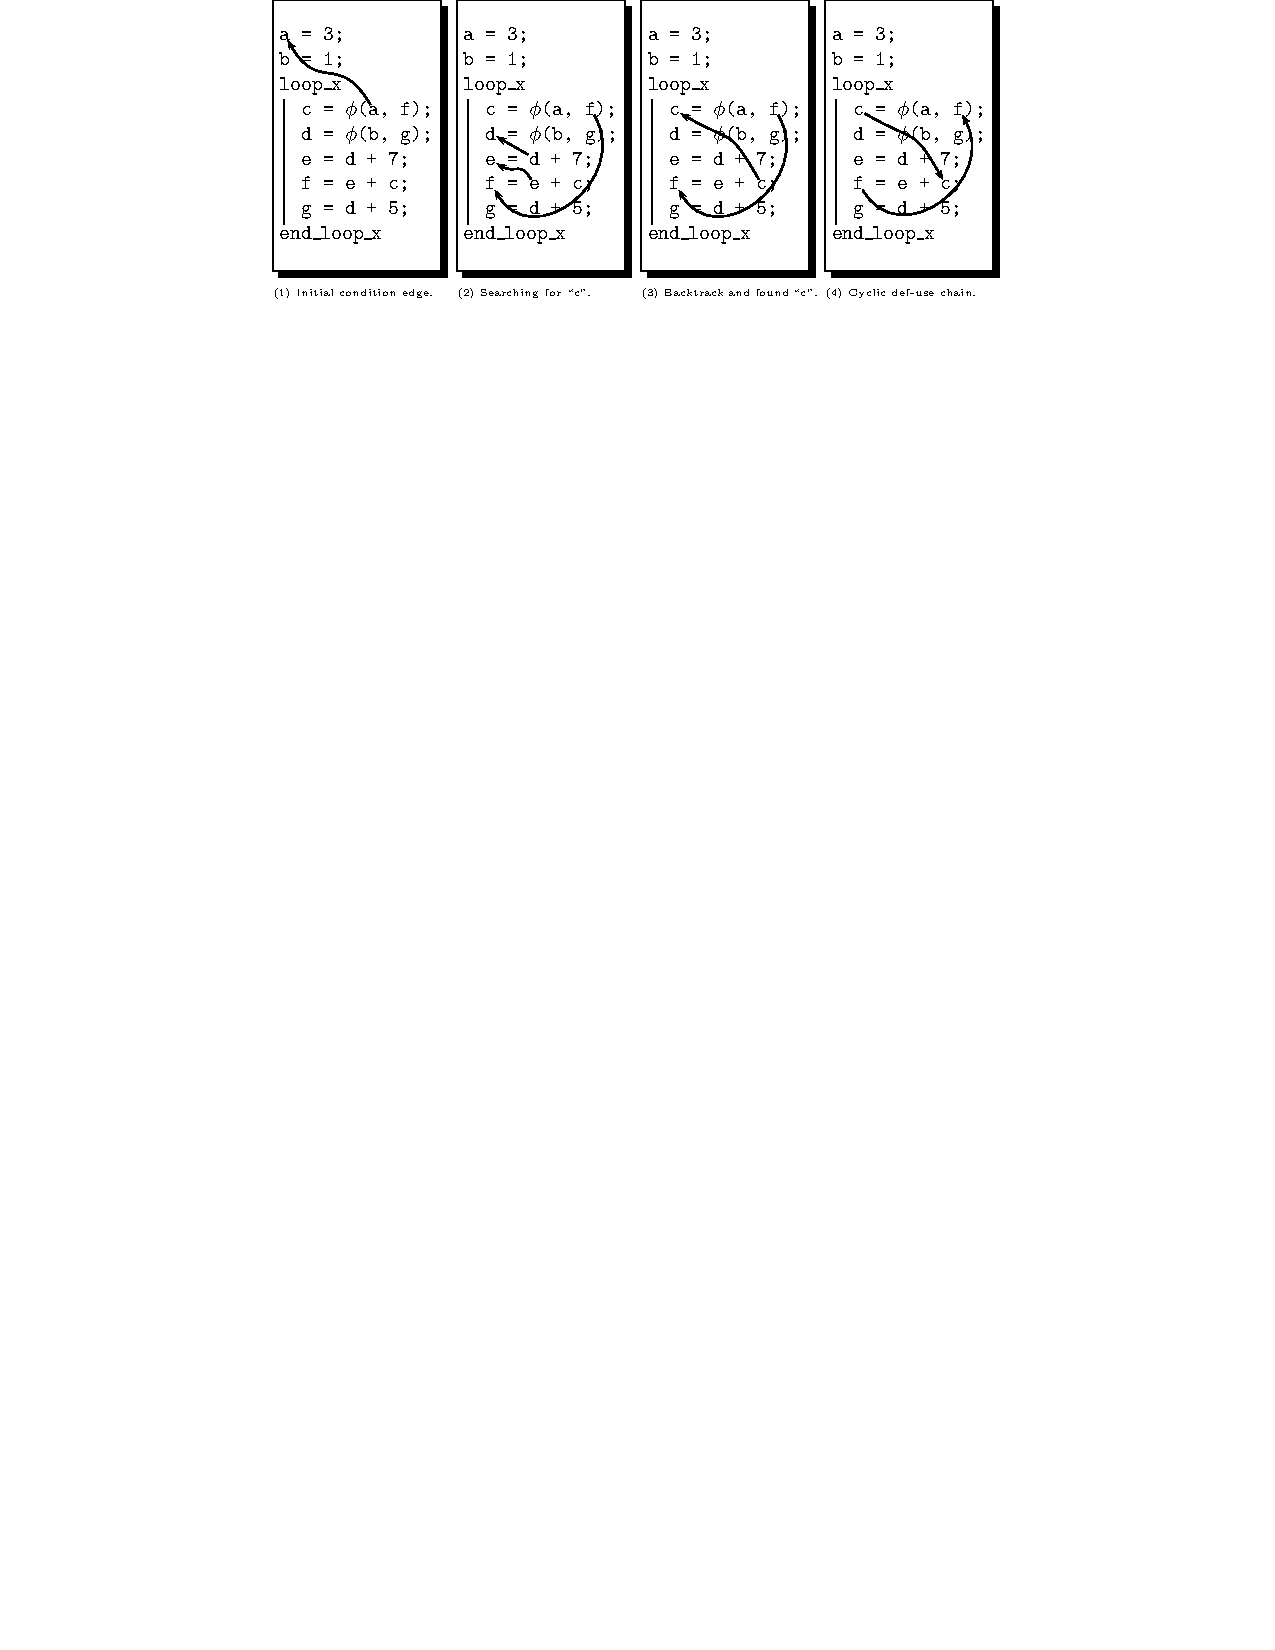
\includegraphics[width=1.2\textwidth]{iv_step}
  \end{center}
  \vspace{-50em}
  \caption{Detection of the cyclic definition using a depth first
    search traversal of the use-def chains.}
  \label{spop:fig:ivstep}
\end{figure}

Let's now look at an example, presented in Figure~\ref{spop:fig:ivstep},
to see how the stride detection works.  The arguments of a $\phi$-node are
analyzed to determine whether they contain self references or if they
are pointing towards the initial value of the induction variable.  In
this example, (1) represents the use-def edge that points towards the
invariant definition.  When the argument to be analyzed points towards
a longer use-def chain, the full chain is traversed, as shown in (2),
until a phi node is reached.  In this example, the phi node that is
reached in (2) is different to the phi node from which the analysis
started, and so in (3) a search starts over the uses that have not yet
been analyzed.  When the original phi node is found, as in (3), the
cyclic def-use chain provides the step of the induction variable: in
this example, the step is ``+ e''.  Knowing the symbolic expression
for the step of the induction variable may not be enough, as we will
see next, one has to instantiate all the symbols (``e'' in the current
example) defined in the varying loop to precisely characterize the
induction variable.

\subsection{Translation to chains of recurrences}

Once the def-use circuit  and its corresponding overall loop
update expression have been identified, it is possible to translate the
sequence of values of the induction variable to a chain of recurrence.
The syntax of a polynomial chain of recurrence is: $\CHREC{base, +,
  step}_x$, where $base$ and $step$ may be arbitrary expressions
or constants, and $x$ is the loop to which the sequence is
associated.  As a chain of recurrence represents the sequence of values
taken by a variable during the execution of a loop, the associated expression of a
chain of recurrence is given by $\CHREC{base, +, step}_x (\ell_x) =
base + step * \ell_x$, that is a function of $\ell_x$,
the number of times the body of loop $x$ has been executed.

When $base$ or $step$ translates to sequences varying in outer
loops, the resulting sequence is represented by a multivariate chain
of recurrences.  For example $\CHREC{\CHREC{0, +, 1}_x, +, 2}_y$
defines a multivariate chain of recurrence with a step of $1$ in loop
$x$ and a step of $2$ in loop $y$, where loop $y$ is enclosed in loop
$x$.

When $step$ translates into a sequence varying in the same loop,
the chain of recurrence represents a polynomial of a higher degree.
For example, $\CHREC{3, +, \CHREC{8, +, 5}_x}_x$ represents a
polynomial evolution of degree $2$ in loop $x$.  In this case,
the chain of recurrence is also written omitting the extra braces:
$\CHREC{3, +, 8, +, 5}_x$.  The semantics of the chains of recurrences
is defined, using the binomial coefficients $\binom{n}{p} = \frac{n!}{p!(n-p)!}$, by the
equation:
\begin{equation*}
  \CHREC{c_0,+,c_1,+,c_2,+,\ldots,+,c_n}_x(\vec{\ell_x})=
  \sum_{p=0}^{n}c_{p}\binom{\ell_x}{p}.
\end{equation*}
with $\vec{\ell}$ the iteration domain vector (the iteration loop
counters for all the loops in which the chain of recurrence variates),
and $\ell_x$ the iteration counter for loop $x$.  This semantics is very useful in the analysis of induction variables, as it
makes it possible to split the analysis into two phases, with a
symbolic representation as a partial intermediate result:
\begin{enumerate}
\item first, the analysis leads to a symbolic form, where the step
  part ``s'' is left in a symbolic form, i.e., $\CHREC{c_0, +, s}_x$;
\item then, by instantiating the step, i.e., $s = \CHREC{c_1, +,
  c_2}_x$, the chain of recurrence is that of a higher degree
  polynomial, i.e., $\CHREC{c_0, +, \CHREC{c_1, +, c_2}_x}_x =
  \CHREC{c_0, +, c_1, +, c_2}_x$.
\end{enumerate}

\subsection{Instantiation of symbols and region parameters}

The last phase of the induction variable analysis consists in the
instantiation (or further analysis) of symbolic expressions left from
the previous phase.  This includes the analysis of induction variables in
outer loops, the analysis of the end value of a loop preceding the
analyzed loop, and the replacement of other definitions occurring before the loop with their corresponding defined expression.  In some
cases, it becomes necessary to leave in a symbolic form every
definition outside a given region, and these symbols are then called
parameters of the region.

Let's look again at the example of Figure~\ref{spop:fig:ivstep} to see
how the sequence of values of the induction variable $c$ is
characterized with the chains of recurrences notation.  The first
step, after the cyclic definition is detected, is the translation of
this information into a chain of recurrence: in this example, the
initial value (or base of the induction variable) is $a$ and the
step is $e$, and so $c$ is represented by a chain of recurrence
$\CHREC{a, +, e}_1$ that is varying in loop number $1$.  The symbols
are then instantiated: $a$ is trivially replaced by its definition
leading to $\CHREC{3, +, e}_1$.  The analysis of $e$ leads to this
chain of recurrence: $\CHREC{8, +, 5}_1$ that is then used in the
chain of recurrence of $c$, $\CHREC{3, +, \CHREC{8, +, 5}_1}_1$ and
that is equivalent to $\CHREC{3, +, 8, +, 5}_1$, a polynomial of
degree two:
\begin{eqnarray*}
  F(\ell)
  &=& 3\binom{\ell}{0} + 8\binom{\ell}{1} + 5\binom{\ell}{2} \\
  &=& \frac{5}{2}\ell{}^2+\frac{11}{2}\ell + 3.
\end{eqnarray*}

\subsection{Number of iterations and computation of the end of loop value}

One of the important properties of loops is their trip count (i.e.,
the number of times the loop body is executed before the exit
condition becomes true).  In simple loops, the exit condition of the
loop is a comparison of an induction variable against some constant,
parameter, or another induction variable.  The number of iterations is
then computed as the (minimum) solution of an (in)equality with integer solutions, also called a Diophantine (in)equality.  When one
or more coefficients of the Diophantine (in)equality are parameters, the
solution is left under a parametric form.  The number of iterations
can also be an expression varying in an outer loop, in which case,
it can be characterized using a chain of recurrence expression.

Consider a scalar variable varying in an outer loop with strides dependent on the value computed in an inner loop. 
The expression representing the number of iterations in the inner loop can then be used to express the evolution function of the scalar
variable varying in the outer loop.

For example, the following code
\begin{verbatim}
x = 0;
for (i = 0; i < N; i++)   // loop_1
  for (j = 0; j < M; j++) // loop_2
    x = x + 1;
\end{verbatim}
would be written in loop closed \SSA{} form as:

\[
\begin{array}{lcl}
  x_0 &=& 0\\
  i &=& \textrm{\loopphi}_1 (0, i + 1)\\
  x_1 &=& \textrm{\loopphi}_1 (x_0, x_2)\\
  x_4 &=& \textrm{\closephi}_1 (i < N, x_1)\\
  j &=& \textrm{\loopphi}_2 (0, j + 1)\\
  x_3 &=& \textrm{\loopphi}_2 (x_1, x_3 + 1)\\
  x_2 &=& \textrm{\closephi}_2 (j < M, x_3)\\
\end{array}
\]
$x_3$ represents the value of variable $x$ at the end of the
original imperative program.  The analysis of scalar evolutions for
variable $x_4$ would trigger the analysis of scalar evolutions for all
the other variables defined in the loop closed \SSA{} form as follows:
\begin{itemize}
\item first, the analysis of variable $x_4$ would trigger the analysis
  of $i$, $N$ and $x_1$
  \begin{itemize}
  \item the analysis of $i$ leads to $i = \CHREC{0, +, 1}_1$ i.e. the canonical loop counter $l_1$ of $loop_1$.
  \item $N$ is a parameter and is left under its symbolic form
  \item the analysis of $x_1$ triggers the analysis of $x_0$ and $x_2$
    \begin{itemize}
    \item the analysis of $x_0$ leads to $x_0 = 0$
    \item analyzing $x_2$ triggers the analysis of $j$, $M$, and $x_3$
      \begin{itemize}
      \item $j = \CHREC{0, +, 1}_2$ i.e. the canonical loop counter $l_2$ of $loop_2$.
      \item $M$ is a parameter
      \item $x_3 = \textrm{\loopphi}_2 (x_1, x_3 + 1) = \CHREC{x_1, +, 1}_2$
      \end{itemize}
    \item $x_2 = \textrm{\closephi}_2 (j < M, x_3)$ is then computed as the last value of $x_3$ after
      $loop_2$, i.e., it is the chain of recurrence of $x_3$ applied
      to the first iteration of $loop_2$ that does not satisfy $j < M$ or equivalently $l_2<M$. The corresponding Diophantine inequality $l_2\geq M$  have minimum solution $l_2=M$. So, to finish the computation of the scalar evolution of
      $x_2$ we apply $M$ to the scalar evolution of $x_3$, leading
      to $x_2 = \CHREC{x_1, +, 1}_2 (M) = x_1 + M$;
    \end{itemize}
  \item the scalar evolution analysis of $x_1$ then leads to $x_1 =
    \textrm{\loopphi}_1 (x_0, x_2) = \textrm{\loopphi}_1 (x_0, x_1 + M) = \CHREC{x_0, +, M}_1 =
    \CHREC{0, +, M}_1$
  \end{itemize}
\item and finally the analysis of $x_4$ ends with $x_4 = \textrm{\closephi}_1 (i
  < N, x_1) = \CHREC{0, +, M}_1 (N) = M * N$.
\end{itemize}


\section{Further reading}
FAB: des copier-coller pour remplir cette partie:\\

As we have seen in this chapter, the \CFG{} representation is embedded
in the \SSA{} structure, and properties of the \CFG{} like the
execution order and the natural loops can be detected by only looking
at the \SSA{} definitions and uses.  The detection of natural loops is
the first step in the analysis of induction variables: after the
detection of self referent definitions, it is practical to use the
chains of recurrences \cite{BWZ94,KMZ98,Zim01} to characterize the
sequence of values taken by a variable during the execution of a loop.
The number of iterations of loops can be computed based on the
characterization of induction variables.  This paves the way to
advanced loop optimizations that need both the number of iterations
and induction variable characterizations.

The computation of the end of loop value can also be used for scalar
optimization purposes, for example in the case of the constant
propagation or the value range propagation after loops.  It enables
more scalar transformations when the induction variable is used after
its defining loop.  Loop transformations also benefit from the
replacement of the end of loop value as this removes scalar
dependencies between consecutive loops.  Another interesting use of the
end of loop value is the estimation of the worst case execution time
(WCET) where one tries to obtain an upper bound approximation of the
time necessary for a program to terminate.

Dans le désordre je pense aux choses suivantes pour mettre dans cette partie:
\begin{itemize}
\item référence concernant la théorie sur les chaines de récurrence
\item référence sur la résolution d'inegalités diophantines. Eventuellement donner des références d'outils.
\item donner des références pour le calcul du nombre de points dans un polyhèdre.
\item référence au papier et/ou la thèse qui contient les pseudo-codes 
\item parler de SCEV qu'il y a dans LLVM (connais pas dixit Albert) et aussi de la technique initiale de Wolf.
\item parler des "extentions" de ce type de technique qui permet entre autre de détecter les réductions (j'ai un papier là dessus je crois mais pas sur. Ca existe clairement dans le monde single assignment à la Feautrier (par Paul lui même je crois). C'est trivial dans le cas scalaire faudrait trouver une référence je pense.
\item je pense que l'on peut parler de toutes les applications liées au calcul de IV. Entre autre la transformation de boucle (whatever le monde polyhedrique) qui nécessite si la variable d'induction est live-out de la boucle de savoir calculer sa valeur de sortie.
\item parler du gated SSA (décrit dans le chapitre vsdg) qui pour pouvoir faire du demand driven implémente aussi une loop-close form.
\item de manière plus générale, la technique de loop-closed form qui encapsule une boucle, permet d'isoler l'effet des transformations effectuées au sein de la boucle. C'est une technique classique utilisée pour simplifier la mise à jour de SSA pour par exemple du loop unrolling ou je crois (à vérifier dans le chapitre associé) de if-conversion.
\end{itemize}
